\subsubsection{Memory Usage}

Charts on Figures \ref{fig:sequential_client_transport_memory}, \ref{fig:parallel_client_transport_memory}, \ref{fig:sequential_server_transport_memory}, and \ref{fig:parallel_server_transport_memory} represent the memory usage of clients and servers during sequential and parallel experiments.

\subsubsection*{Overall Transport Client Memory Usage}

Parallel requests demands more memory than sequential requests. While concurrent requests needs to kep more information in memory at the same time, sequential requests only have to deal with one requests at a time. Thus, the slight increase on memory usage by parallel requests.

\subsubsection*{TLS Memory Usage}

TCP+TLS and QUIC used more memory than TCP. They have to implement all features required by TLS, such as TLS handshake and encryption. Thus, demanding more memory to perform these operations in exchange for encrypted payload.

QUIC used more memory when compared to TCP+TLS, however. It has to deal with more features beyond TLS' requirements, such as sending and receiving UDP packets, and maintaining the QUIC state. Thus, it has increased memory usage.

\clearpage

\begin{figure}[h!]
    \centering
    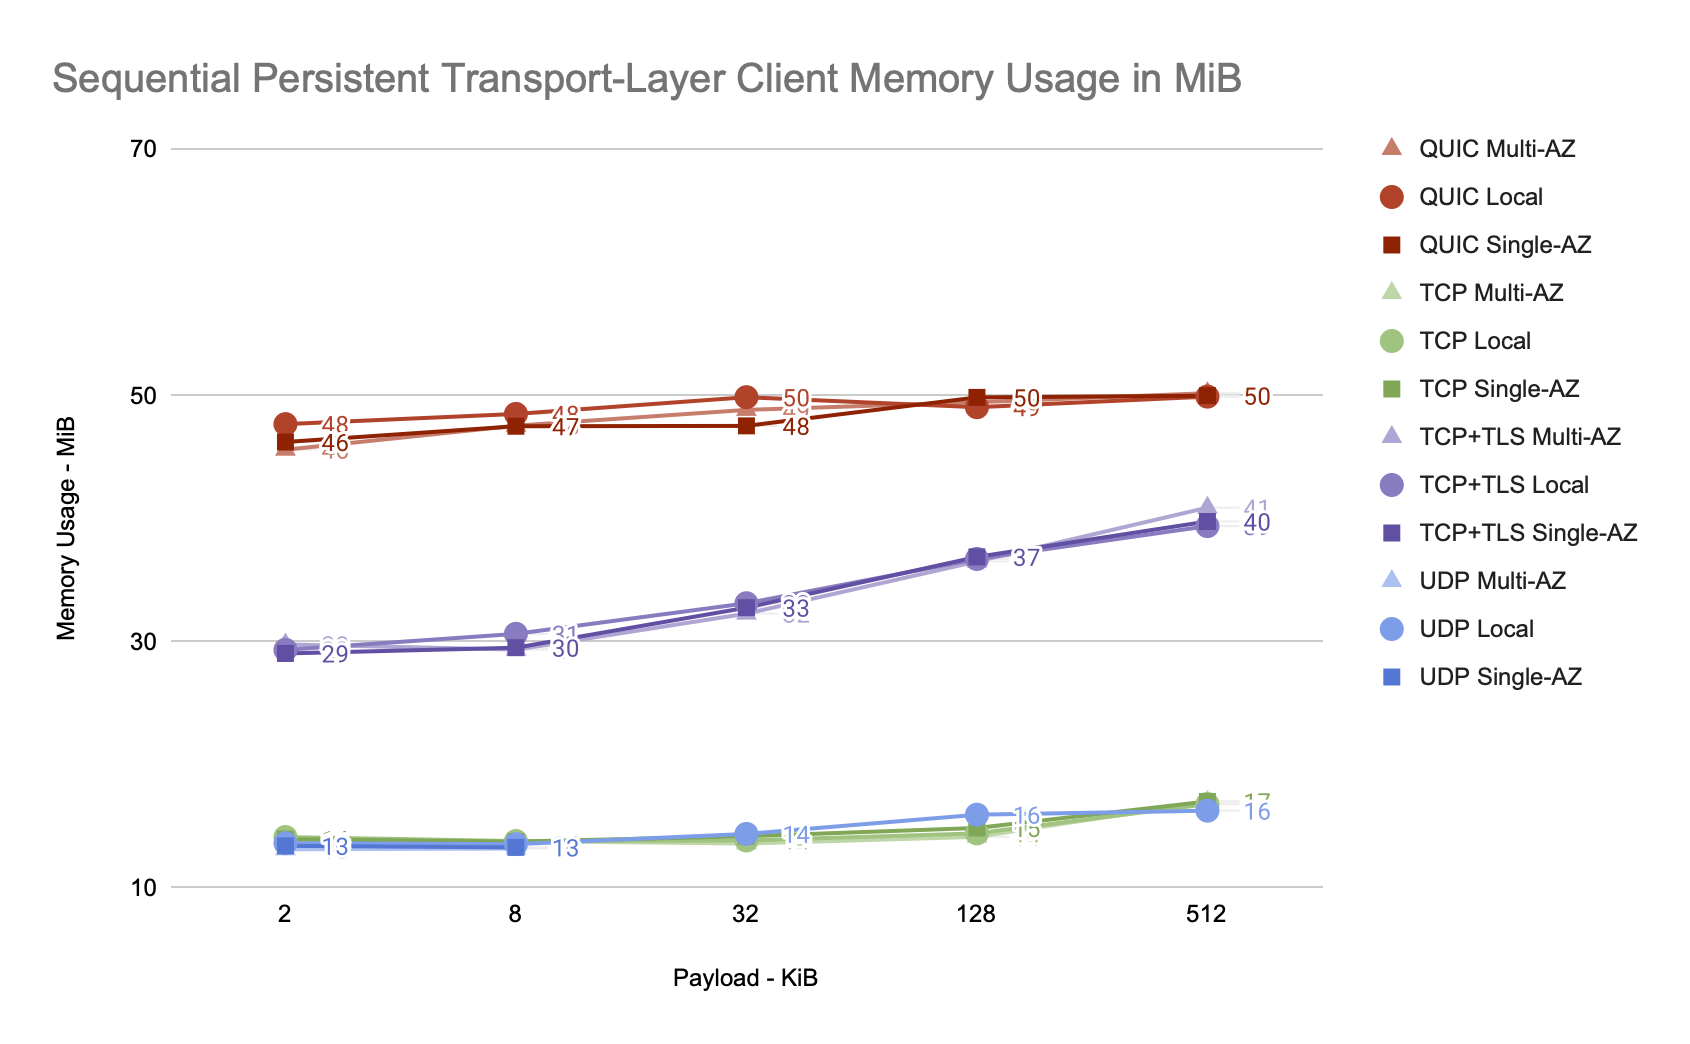
\includegraphics[width=\linewidth]{figures/charts/Sequential Persistent Transport-Layer Client Memory Usage in MiB.png}
    \caption{Sequential Persistent Transport-Layer Client Memory Usage in MiB}
    \label{fig:sequential_client_transport_memory}
\end{figure}
\begin{figure}[h!]
    \centering
    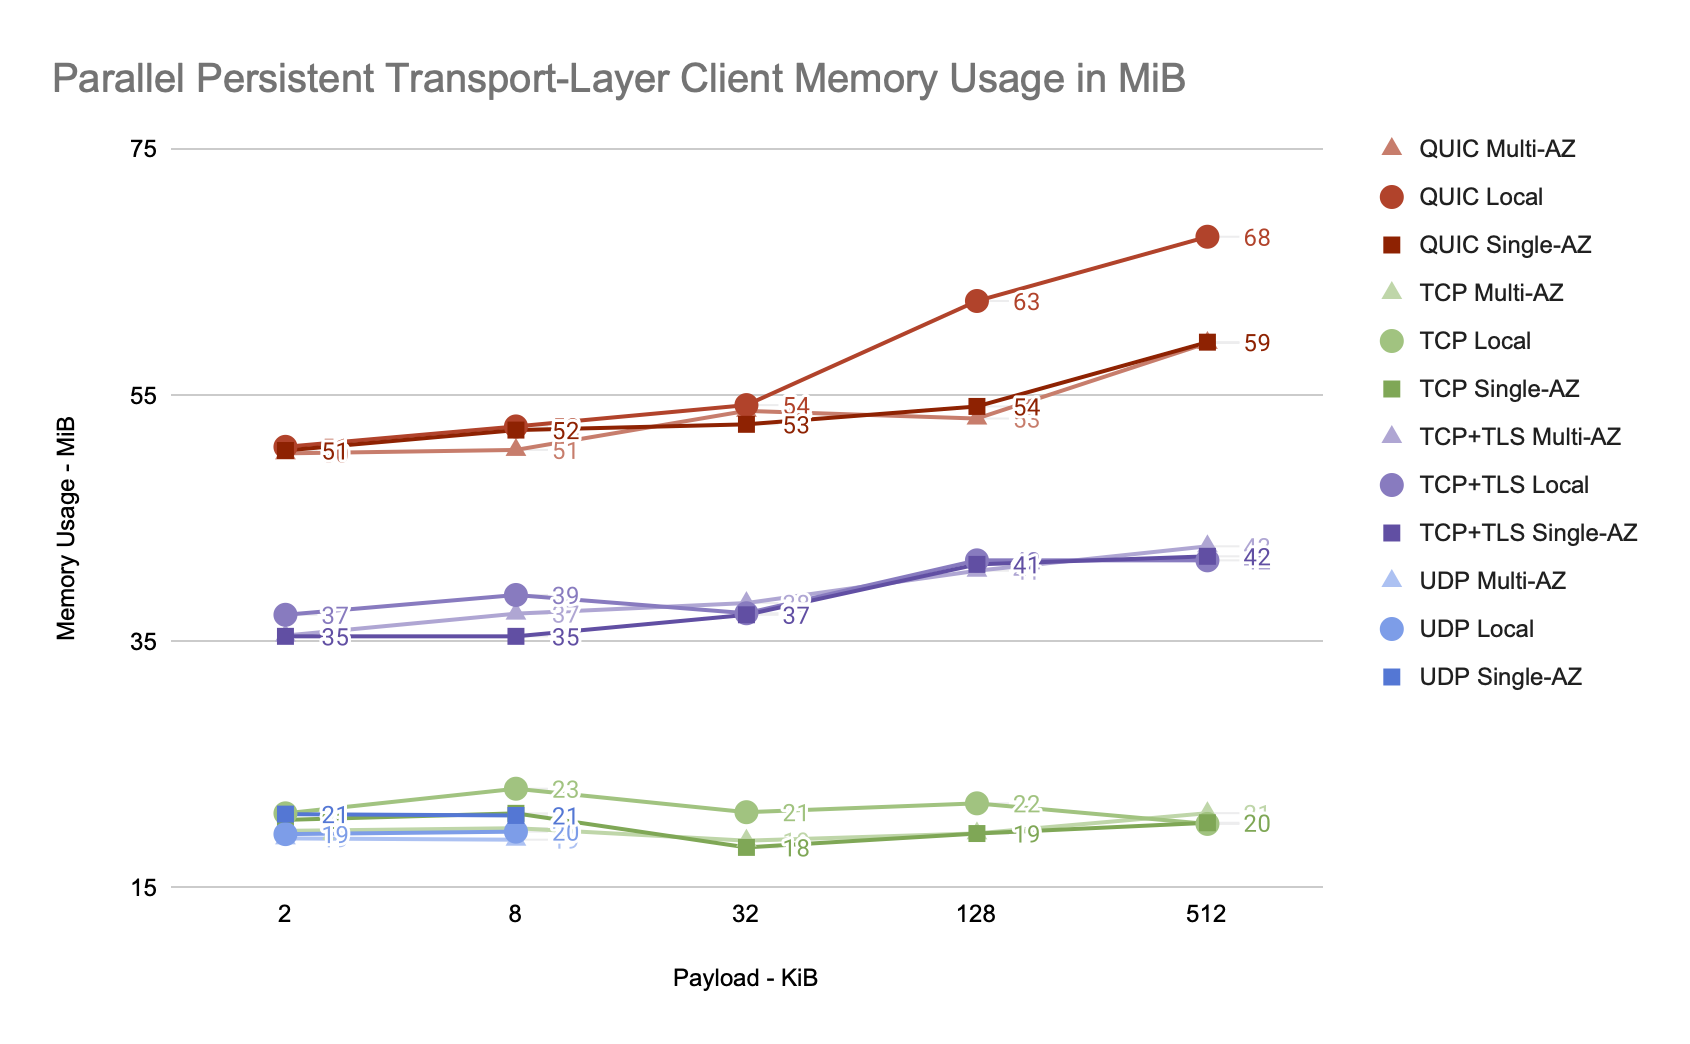
\includegraphics[width=\linewidth]{figures/charts/Parallel Persistent Transport-Layer Client Memory Usage in MiB.png}
    \caption{Parallel Persistent Transport-Layer Client Memory Usage in MiB}
    \label{fig:parallel_client_transport_memory}
\end{figure}

\begin{figure}[h!]
    \centering
    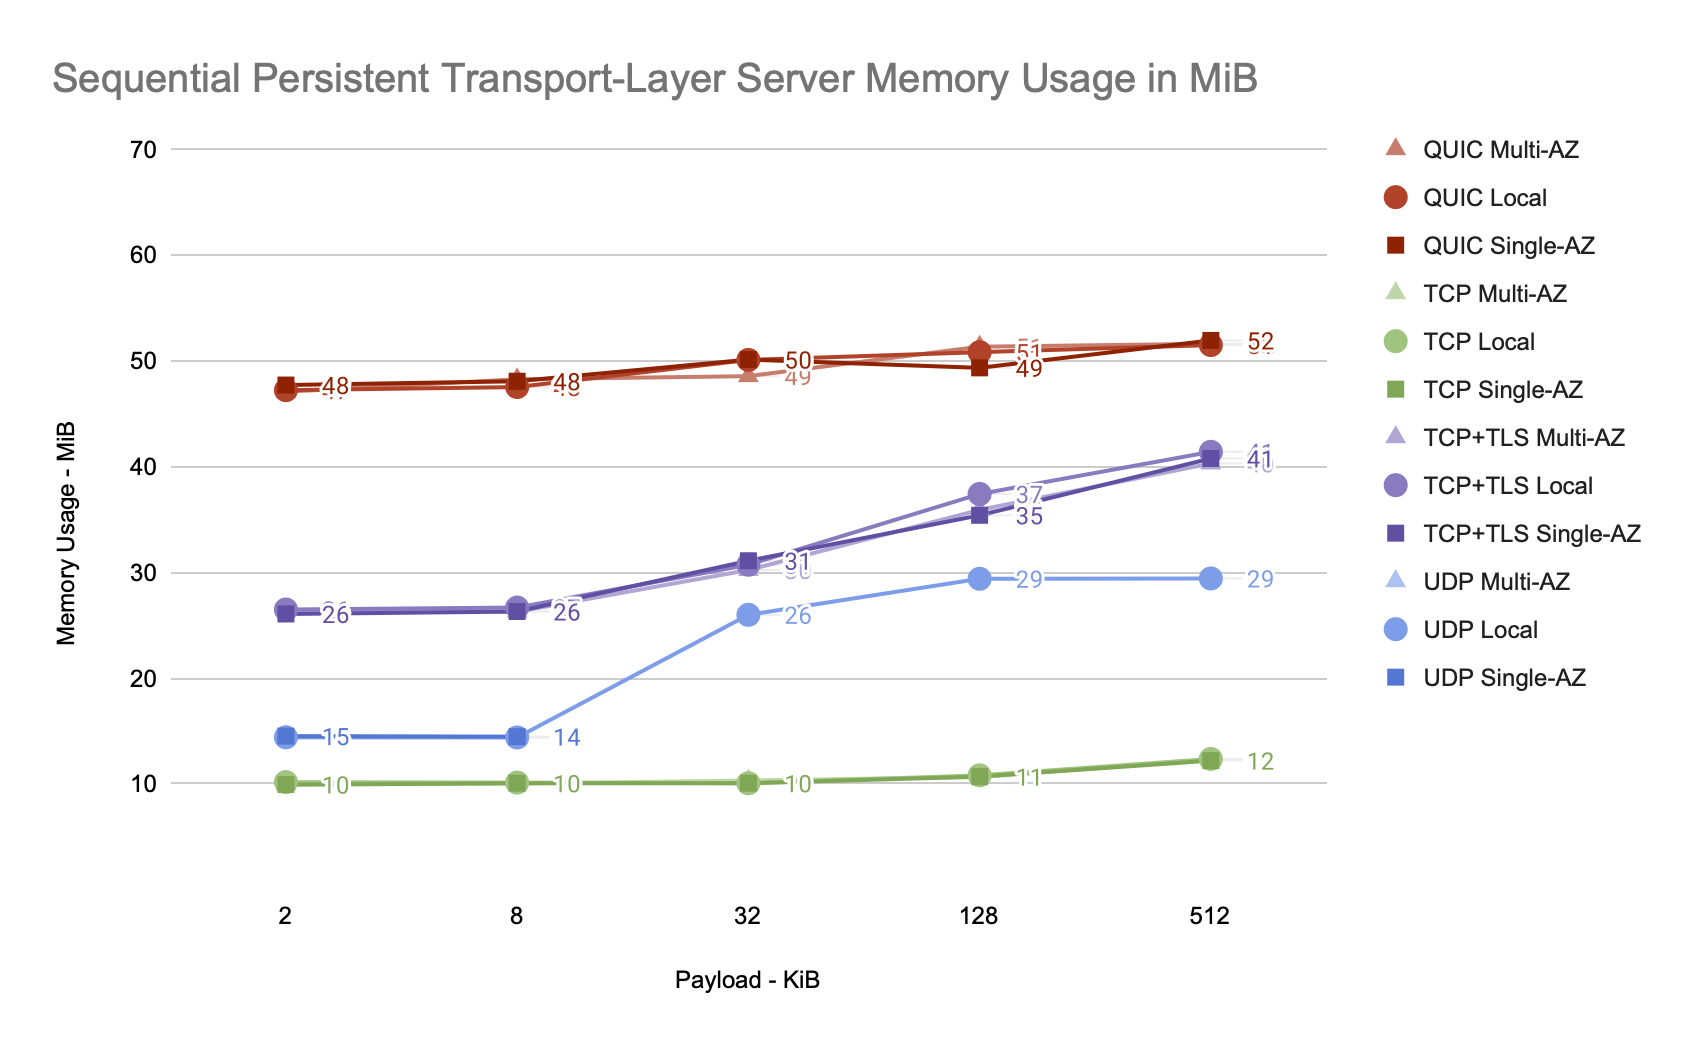
\includegraphics[width=\linewidth]{figures/charts/Sequential Persistent Transport-Layer Server Memory Usage in MiB.png}
    \caption{Sequential Persistent Transport-Layer Server Memory Usage in MiB}
    \label{fig:sequential_server_transport_memory}
\end{figure}
\begin{figure}[h!]
    \centering
    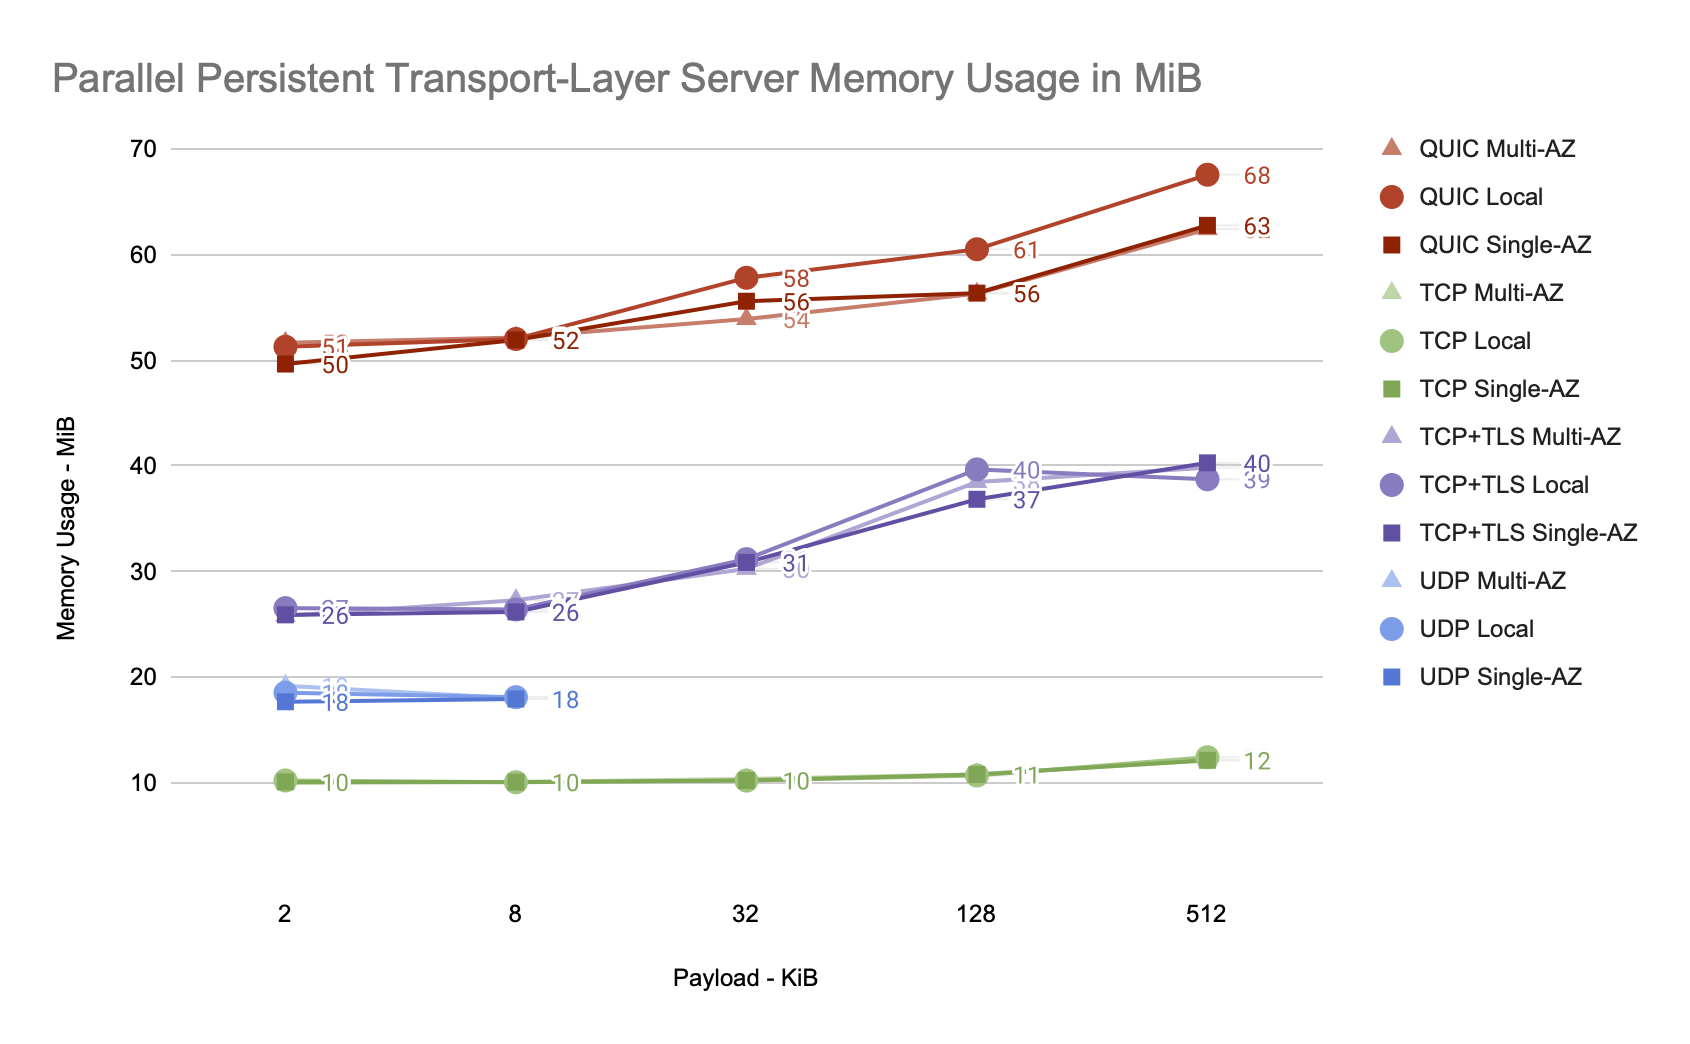
\includegraphics[width=\linewidth]{figures/charts/Parallel Persistent Transport-Layer Server Memory Usage in MiB.png}
    \caption{Parallel Persistent Transport-Layer Server Memory Usage in MiB}
    \label{fig:parallel_server_transport_memory}
\end{figure}
